The dependency directed graph (\emph{DDG}) $G=(V,A)$ is made of a set of vertices $V$ representing the non-fixed 
variables, invariants and the non transformed constraints. The vertex $v \in V$ has an outgoing arc to vertex $u \in V$ 
if and only if the value of the variable corresponding to $u$ is directly dependent on the value of variable 
corresponding to $v$. The variable vertices only have outgoing arcs and the constraints can only have ingoing arcs. 
\boste{Skal det stå her efter omstrukturering} The initial model will be modified by introducing invariants defined by 
oneway constraints and vertices representing invariants will be added to the graph $G$. \\
The graph can be illustrated with all the variable vertices to the left with outgoing arcs going right to vertices 
representing invariants and constraints.  \\  
The invariants are variables that are defined by oneway constraints or they can be auxiliary variables used in the local 
search. If a variable is defined by a oneway constraint the variable vertex is removed from $G$ since the value of that 
variable is given by the invariant representing it. \\  
%From now on when talking about vertices in $G$ it refers to the variable, invariant or constraint it represents unless 
%other stated. \\
%The variables are non-fixed and non-defined and only have outgoing arcs. 
%Variables and invariants has an outgoing arc to the invariants that 
%depends on their value. \\ 
The DDG is used to update values of variables and invariants during local search. The graph $G$ is used to build the 
propagation queues described in subsection \ref{sec_propaqueue}. \\
The example is a model with three variables and a two constraint and will illustrate how a possible dependency directed 
graph $G$ is made. 
\begin{center}
\begin{tabular}{rlr}
$ c_1: $&$2x_1 + x_2 - x_3 $&$= 2$ \\
$ c_2: $&$x_2 + x_3 $&$\leq 1$ \\
\end{tabular} 
\end{center}
$G$ consist of the three variables $x_1$, $x_2$, and $x_3$ and the constraints $c_1$ and $c_2$. The 
variable $x_3$ can be defined as an invariant $inv_1$ by transforming $c_1$ to a oneway constraint. Once 
variable $x_3$ is defined by a oneway constraint $c_1$ and $x_3$ are removed from the graph and replaced by invariant 
$inv_1$. The variables $x_1$ and $x_2$ defines $inv_1$ hence they have outgoing arcs to $inv_1$. Invariant $inv_1$ has 
an outgoing arc to $c_2$ since Variable $x_3$ participates in $c_2$. \\
\begin{figure}[b]
\begin{center}
    \begin{tikzpicture}[scale=1]
        \vertex[label=$x_1$](x1) at (0,2) {};
        \vertex[label=$x_2$](x2) at (0,0) {};
        \vertex[label=$inv_1$](i1) at (2,1) {};
        \vertex[label=$c_2$](c2) at (4,0) {};

    \tikzset{EdgeStyle/.style={->}}
        \Edge(x1)(i1)
        \Edge(x2)(i1)
        \Edge(x2)(c2)
        \Edge(i1)(c2)
        %\Edge(y1)(c3)
        %\Edge(y2)(c3)
    \end{tikzpicture}
        \captionof{figure}{Small example of DDG}
    \label{fig_smallG}
\end{center}
\end{figure} \noindent
Auxiliary variable can be useful to update constraint violations and in this example we could create an auxiliary 
variable where value is the sum of the left hand side of $c_2$. The auxiliary variable will be represented 
by an invariant $inv_2$ which will be added to $G$. The invariant $inv_1$, representing $x_3$, and variable $x_2$ have 
an outgoing arc to $inv_2$ that has an outgoing arc to $c_2$.
\begin{figure}[b]
\begin{center}
    \begin{tikzpicture}[scale=1]
        \vertex[label=$x_1$](x1) at (0,2) {};
        \vertex[label=$x_2$](x2) at (0,0) {};
        \vertex[label=$inv_1$](i1) at (2,1) {};
        \vertex[label=$inv_2$](i2) at (4,0) {};
        \vertex[label=$c_2$](c2) at (6,0) {};

    \tikzset{EdgeStyle/.style={->}}
        \Edge(x1)(i1)
        \Edge(x2)(i1)
        \Edge(x2)(i2)
        \Edge(i1)(i2)
        \Edge(i2)(c2)
    \end{tikzpicture} 
    \captionof{figure}{Small example of DDG continued}
    \label{fig_smallG2}
\end{center}
\end{figure}   \label{fig_smallG} 
When changing the value of $x_2$ both invariants need to be updated since they are dependent on the value of $x_2$. 
Invariant $inv_2$ is dependent on the value of $inv_1$ therefore to avoid updating $inv_2$ twice, it is beneficial to 
update 
$inv_1$ before updating $inv_2$. This is the ordering given the propagation queue that is discussed in the next 
subsection. \medskip \\
%\end{minipage}
%\boste{start on algorithms}
%The DDG $G$ is initially a bipartite graph where all the decision variables $X$ are vertices in one set and all the 
%constraints $C$ are vertices in the other set. If constraint $c$ applies to a variable $x$ then there is an arc from 
%the vertex representing $x$ to the vertex representing $c$. \\   
In order to avoid circular definitions of invariants dependency directed graph $G$ should be acyclic. A circular 
definition could be if $x_i$ is used to define $x_j$ and vise versa. Then a change in value 
of $x_i$ would lead to a change in value of $x_j$ that again changes the value of $x_i$ and so on. \\ 
Once all invariants are introduced, all strongly connected components of size two or more in $G$ is found. A 
\emph{strongly connected component} (SCC) is a maximal set of vertices $V^{SCC}$ such that for each pair of vertices 
$(u,v) \in V^{SCC}$ there exist both a path from $u$ to $v$ and a path from $v$ to $u$ \cite[p. 1170]{cormen}. 
To find all SCC of size two or more Tarjan's algorithm \boste{cite SIAM J. Comput., 1(2), 146–160.} that finds strongly 
connected components (\emph{SCC}) is used. \boste{Description of Tarjan and timestamps} \\ 
Each of these strongly connected components must be broken in order to keep $G$ acyclic, since a SCC consist of at 
least one cycle. A SCC can be broken by removing arcs and/or removing vertices. The arcs $A$ represent relations 
between variables, invariants and constraints and should not be changed. The vertices $V^{SCC}$ can only be vertices 
representing invariant since variable only have outgoing arcs and constraint only have ingoing arcs. Undefining one of 
those invariants corresponds to removing one of the vertices, hence breaking the SCC. An invariant can be undefined by 
reintroducing the variable it represents and removing the invariant from the model. The oneway constraint used to 
define the invariant is transformed back into a functional constraint again and is reintroduced in the model. \\
For each SCC one of the vertices is chosen and the invariant it represents is undefined. The invariant is chosen in the 
order of lowest domain then highest arity of oneway constraint defining it \boste{Search priority?}. If there is ties 
they are broken at random.  \\  
Once these strongly connected components are broken there is still no guarantee that $G$ is a directed acyclic graph 
(DAG). A strongly connected component can be made of several cycles and it might not be sufficient just to break all 
SCC found by Tarjans algorithm initially. The process of finding SCC with Tarjans algorithm and then 
breaking these strongly connected components is repeated until no strongly connected components (of size two or more) 
is found by Tarjans algorithm. \medskip \\  
The first tiebreaker in algorithm \ref{algo_makeoneway} is used as a heuristic to reduce the number of cycles 
generated. If invariants are not used to define other invariants no cycles can occur, since cycles can only be made of 
invariant vertices. \\
Tarjans algorithm also gives each vertex representing invariants a time stamp that is used to create the propagation 
queues described in the next subsection.  \boste{This should be described earlier} \\




%A circular definition could be if $x_i$ is used define $x_j$ and conversely \boste{vise versa?} then a change in value 
%of $x_i$ would lead to a change in value of $x_j$ that again changes the value of $x_i$ and so on. \\
%Cycles are found with . For each of the 
%strongly connected components of size two or more one of the vertices should be removed. Removing a vertex corresponds 
%to undefine an invariant and reintroduce the transformed constraint. After removing one vertex for each scc Tarjans 
%algorithm is used to find new scc if any. This is repeated until no scc of size two or more is found. Tarjans 
%algorithm 
%is modified a bit to give each vertex a time stamp when it becomes a part of a scc hence the last time it is visited. 
%This time stamp can be used for a topological sorting of the vertices once $G$ is a directed acyclic graph 
%(\emph{DAG}). 
%It gets complicated to compute the propagation queues if there exist a strongly connected component in $G$. 
%Only invariant vertices can be part of a strongly connected component of size at least two, since variables vertices 
%only have outgoing arcs and constraint vertices only have ingoing arcs. This indicates that there could be circular 
%definition of variables. Because of this we want to avoid ending up with strongly connected components in the graph 
%$G$. \medskip \\
%This is not the most efficient way of finding cycles, an algorithm with better complexity is described by \boste{cite 
%SIAM J. Comput., 4(1), 77–84, Tarjan has complexity O(|V|+|A|) not sure it is actually better to find elementary 
%cycles. Talk about finding minimum number of vertices to remove. Minimum feedback, NP-hard}. \\ 


%Consider the following three constraints as a small example. \boste{Should the example be introduced before the 
%algorithms?}
%\begin{center}
%\begin{tabular}{rlr}
%$ c_1: $&$2x_1 + y_2 -y_1 $&$= 2$ \\
%$ c_2: $&$2x_1 - y_2 $&$= 2 $ \\ 
%$ c_3: $&$x_1 +y_1 +y_2 $&$\leq 5 $
%\end{tabular} 
%\end{center}
%At first $y_1$ cannot be defined by a \oneway but $y_2$ can be defined by $c_2$ and then $y_1$ can be defined by 
%$c_1$. 
%The order in which the \oneway are created matters. \boste{Not finished here, continue tomorrow morning} 
%\begin{center}
%    \begin{tikzpicture}[scale=1]
%        \vertex[label=$x_1$](x1) at (-1,1) {};
%        \vertex[label=$y_1$](y1) at (3,2) {};
%        \vertex[label=$y_2$](y2) at (1,0) {};
%        %\vertex[label=$c_3$](c3) at (5,1) {};
%         %\vertex[label=$c_2$](c2) at (5,0) {};
%    \tikzset{EdgeStyle/.style={->}}
%        \Edge(x1)(y1)
%        \Edge(y2)(y1)
%        \Edge(x1)(y2)
%        %\Edge(x1)(c3)
%        %\Edge(y1)(c3)
%        %\Edge(y2)(c3)
%    \end{tikzpicture}
%\end{center}

%algorithm \ref{algo_defintvar} first check if $y_1$ can be defined by a \oneway which it cannot since $c_1$ applies to 
%two integer variables. Then $y_2$ cannot be defined by $c_1$ but can be defined by $c_2$. Then $c_2$ is transformed 
%into a \oneway $c_2'$ that defines $y_2$ and it is added to the DDG $G$, $c_2: y_2 = 2x_2 -2$. T  


% \floatname{algorithm}{Finding One-way constraints}
%\begin{algorithm}[ht]
% \caption{O$(|V|^2C_{mav}$O$($\method{canBeMadeOneway()}$)$}
% \begin{algorithmic}\label{updateGraph1}
%  \STATE{$Q = \emptyset$}
%  \STATE{$V = $ model.getVariables()}
%  \STATE{V.sort()}
%  \STATE{\bool change = \true }
%  \WHILE{change}
%    \FOR{\var var in $V$}
%      \FOR{\cons cons in var.usedInConstriant()}
%	\IF{\method{canBeMadeOneway(var, cons)}}
%	  \STATE{V.remove(var)}
%	  \STATE{$Q.psuhback($var$)$}
%	  \STATE{\Break }
%	\ELSE
%	\STATE{change = \\false}
%	\ENDIF
%      \ENDFOR
%    \ENDFOR
%   % \STATE{laxer$++$}
%%{$j\leftarrow 1$ \TO $i-1$}
%  \ENDWHILE
% \end{algorithmic}
%
%\end{algorithm}


% \floatname{algorithm}{}
%\begin{algorithm}[ht]
% \caption{\bool \method{canBeMadeOneway}(\var \text{var}, \cons cons) \qquad O$(V_{mav} + $O$($\method{makeOneway}$))$}
% \begin{algorithmic}\label{updateGraph1}
% \IF{cons.isOneway()}
%  \RETURN \\false
%  \ENDIF
% \STATE{\Int notDefined = 0} 
% \FOR { \var v in cons.getVariables}
% \IF{v.isInteger()}
%  \IF{!v.isDefinedBxOneway}
%  \STATE{notDefined++}
%  \ENDIF
%  \ENDIF
%  \IF{notDefined $> 1$}
%    \RETURN \\false  
% \ENDIF
% \ENDFOR
% \STATE{\Int coef = var.getCoefficient(cons)}
% \STATE{\Int objCoef = var.getObjectiveCoefficient()}
% 
% \IF{cons.Relation = EQ \OR coef$\cdot$objCoef $< 0$}
%    \STATE{\method{makeOneway}(\var var, \cons cons)}
%    \RETURN \true
% \ENDIF
% \RETURN \\false
% \end{algorithmic}
%\end{algorithm}


% \floatname{algorithm}{}
%\begin{algorithm}[ht]
% \caption{\method{makeOneway}(\var \text{var}, \cons cons) \qquad O$(V_{mav})$}
% \begin{algorithmic}\label{updateGraph1}
% \STATE{variables = cons.getVariables()-var}
% \STATE{coefficients = cons.getCoefficient-var.coefficients}
% \STATE{\Int coef = var.getCoefficient(cons)}
% \IF{coef $\neq$ -1}
% \STATE{coefficients = $\frac{-1}{coef}\cdot$ coefficients}
% \ENDIF
% \STATE{\invar invar$(variables, coefficients)$}
% \FOR{\var v in variables}
%  \IF{v.isDefinedBxOneway}
%    \STATE{\invar inv = v.oneway}
%    \STATE{inv.updateList.pushback(invar)}
%  \ELSE
%  \STATE{v.updateList.pushback(invar)}
%  \ENDIF
%   \ENDFOR
%   \STATE{cons.isOneway = \true }
%   \STATE{cons.defines = invar }
%   \STATE{var.setDefinedBx(invar,cons)}
%   \STATE{model.add(invar)}
%   \STATE{invar.currentvalue = -cons.getArgument(1)} 
% \end{algorithmic}
%\end{algorithm}
  

%First all integer variables $Y$ in the CSOP $\mathbb{P}$ \boste{Should I call the models CSOP or just model?} get 
%defined by oneway constraints by algorithm \ref{algo_makeints}. If some of the integer variables cannot be defined 
%\boste{Currently report fail and exit}. 
%\\ 
%\IncMargin{1em}
%\begin{algorithm}[H]
%\SetKwData{Oneway}{oneway}
%\SetKwFunction{makeIntVarOneway}{makeIntVarOneway}
%\SetKwFunction{Next}{next}\SetKwFunction{Constraints}{Constraints}\SetKwFunction{Remove}{remove}
%\SetKwFunction{intVarCanBeMadeOneway}{intVarCanBeMadeOneway}
%\algdata 
%\Input{A set $Y$ of integer variables sorted by decreasing domain size}
%\Output{A CBLS model for local search}
%\BlankLine

%\Bool $change = $ \true\;
%\While{$Y \neq \emptyset$ \textbf{and} $change$}{
%  $change = $\false \;
%  \ForEach{$y_i \in Y$}{
%    \upshape select \Var $y_i$ \upshape from $Y$\;
%    \ForEach{\Con $c_j$ \upshape in $C(y_i)$}{
%      \If{\intVarCanBeMadeOneway{$y_i$,$c_j$}}{
%	\makeIntVarOneway{$y_i$,$c_j$}\;
%	Remove $y_i$ from $Y$\;
%	isOneway($c_j$) = \true \;
%	$change = \true$\;
%	\bre\;
%      }
%    }
%  } \label{false}
%}
%\caption{Defining integer variables by one-way constraints}\label{algo_makeints}
%\end{algorithm}\DecMargin{1em}
%\noindent
%For each of the variables $y_i$ each of the constraints $c_j$ that applies to $y_i$ is checked if it can be made 
%oneway 
%to define $y_i$ until one is found or none can be found. This is done until there are no integer variables left or the 
%remaining integer variables cannot be defined, when the boolean change is false after line \ref{false}. Algorithm 
%\ref{algo_checkintoneway} checks if constraint $c_j$ can be made oneway to define $y_i$ and algorithm 
%\ref{algo_makeintoneway} transforms $c_j$ into a oneway constraint defining $y_i$ and updates the DDG $G$. \\
%Let $\mathcal{F} = \{f_1,f_2,\dots ,f_k\}$ be the family of objective functions. \\
%\IncMargin{1em}
%\begin{algorithm}[H]

%\SetKwFunction{relation}{relation}\SetKwFunction{coeff}{coefficient}
%\SetKwFunction{objcoeff}{objectiveCoefficients}
%\algdata
%\Input{\Var $y_i$ and \Con $c_j$}
%\Output{Boolean}
%\BlankLine
%\If{$c_j$ \upshape already defines a oneway constraint}{\Return{} \false\; \boste{This constraint could be removed in 
%$O(\alpha(c_j))$}}

%int $undefinedIntVar = 0$ \;
%\ForEach{\Var $x$ \upshape in $c_j$}{
%  \If{x is undefined integer variable}{
%    $undefinedIntVar++$\;
%  }
%}
%\If{$undefinedIntVar > 1$ \label{undefined}}{\Return{} \false  \boste{Insures no cycle is created} \; 
%\tcp {else only $y_i$ is undefined integer variable}} 
%\If{$c_j$ \upshape is linear equality}{\Return{} \true}
%\If{\upshape coefficient $c_{ij} \geq 0 $ \label{positivecoef}}{ 
%  \Return{} \false \; 
%}
%\ForEach{ $f_j$  in $\mathcal{F}$ }{
% \If{$f_ij < 0$ \label{objectivecoef}}{
%    \Return{} \false \;
%    \boste{Not sure of to define coefficients in objective functions. coefficient of variable i in constraint j could 
%be $c_{ij}$ but $c_j$ is used for constraint and then all variable $y_i$ should be $y_i$}
%  }
%}
%\Return{} \true\;
% \caption{intVarCanBeMadeOneway( \textsf{Variable} $y_i$, \textsf{Constraint} $c_j$)} \label{algo_checkintoneway}
% \caption{Test if a constraint $c$ can define a variable $x$ } \label{algo_checkoneway}
%\end{algorithm}
%\DecMargin{1em}
%If constraint $c_j$ already defines another variable it cannot be used to define $y_i$. Line \ref{undefined} makes 
%sure 
%that integer variable $y_i$ is not defining another integer variable $y_k$. This limits the model and increases the 
%complexity of algorithm \ref{algo_makeints} because of the addition of the initial while loop. The 
%condition in line \ref{undefined} makes sure that no strongly connected component of size 2 or greater is created in 
%$G$. \boste{This should be described why we dont want that and what a SCC is}. The lines \ref{positivecoef} and 
%\ref{objectivecoef} returns false if the coefficient of $y_i$ in $c_j$ is positive or one of the coefficients in the 
%objective functions is negative. If that is not the case the constraint $c_j$ can define variable $y_i$ since we 
%restrict the lower bound of $y_i$ by the oneway constraint and want to minimize its value in the objective functions. 
%This gives some other complications which will be described after algorithm \ref{algo_makeintoneway}. \\ 
%\IncMargin{1em}
%\begin{algorithm}[H]
%\algdata
%\Input{\Var $y_i$ and \Con $c_j$}
%\Output{Updated $G$}
%\BlankLine
%%\int $coef = A_{c,x}$\;
%set $Q$ \tcp*[r]{new coefficient set}
%set $U$ \tcp*[r]{new variable set}
%\tcp{Move $y_i$ to right hand side and set coefficient to 1}
%\ForEach{$x_k$ \upshape in $X(c_j)\setminus {y_i}$}{
%  $c'_{kj} = -\frac{c'_{kj}}{c_{ij}}$ \;   
%  $Q = Q\cup c'_{kj}$ \;
%  $U = Q\cup x_k$ \;
%}
%\tcp{Move right hand side to left hand side and update coefficient}
%double $b' = \frac{B(c_j)}{c_{ij}}$ \;
%\boste{coefficients can now be doubles (non integer)} \;
%\If{$c_j$ \upshape is linear equality}{
%  \textbf{invariant} $inv = $ new \Sum($U$,$Q$,$b'$)\;
%  $G$ = $G \cup \{inv\}$\; 
%  $G$ = $G \setminus \{c_j\}$\; 
%  %\boste{Maybe remove $c$ from $G$}
%  %\Return{\Sum{$V(c)$,$A(c)$,b}}
%} \Else {
%    \boste{Remember to say all constraints are either LQ or EQ} \;
%    \textbf{invariant} $ inv= $ new \Sum($U$,$Q$,$b'$)\;
%    \textbf{Invariant} $ inv' = $ new \Max{$inv$,lowerbound($y_i$)}\;
%    $G$ = $G \cup inv$\; 
%    $G$ = $G \cup inv'$\; 
%    $G$ = $G \setminus \{c_j\}$\; 
% \boste{Maybe remove $c$ from $G$}
  %\Return{\Max{inv,b}}
%}

% \caption{makeIntVarOneway(\textsf{Variable} $y_i$, \textsf{Constraint} $c_j$)} \label{algo_makeintoneway}
% %\caption{Make one-way constraint from $c$ defining variable $x$ } \label{algo_makeoneway}
% \end{algorithm}\DecMargin{1em} \noindent 
%If the constraint $c_j$ is a linear equality constraint, an invariant $inv$ is defined by a new oneway constraint. The 
%oneway constraint is made by isolating $y_i$ on the right side in $c_j$. Then $inv$ is added to $G$ and $c_j$ is 
%removed from $G$. \\ 
%If $c_j$ is not a linear equality constraint then it is a linear constraint with an upper bound $B(c_j)$. Since 
%$c_ij$, 
%the coefficient of $y_i$, in $c_j$ is negative $y_i$ can be isolated on the right hand side as an upper bound. The 
%coefficients of $y_i$ in the objective functions are non-negative, know from algorithm \ref{algo_checkintoneway} line 
%\ref{objectivecoef}. Variable    


